\documentclass[a2paper]{scrartcl}

\usepackage[english]{babel}

\usepackage[utf8]{inputenc}

\usepackage{color}


\usepackage{cite}

\usepackage{nicefrac}

\usepackage{amsmath}
%\allowdisplaybreaks
\usepackage{amssymb}


\usepackage[matrix,arrow]{xy}

\usepackage{tikz}
\usetikzlibrary{calc}

\usepackage{dsfont}
\newcommand{\R}{\mathds{R}}
\newcommand{\Z}{\mathds{Z}}
\newcommand{\csd}{\text{csd}}
\renewcommand{\div}{\text{Div}}
\renewcommand{\hom}{\text{Hom}}
\newcommand{\err}{\text{Err}}
\newcommand{\id}{\text{Id}}
\newcommand{\D}{\text{D}}
\renewcommand{\d}{\mathrm{d}}
\newcommand{\exd}{\mathbf{d}}
\newcommand{\argmin}{\operatornamewithlimits{argmin}}
\newcommand{\sgn}{\mathop{\mathrm{sgn}}\nolimits}
\newcommand{\formpunkt}{\,\text{.}}
\newcommand{\formkomma}{\,\text{,}}
\newcommand{\formtext}[1]{\quad\text{#1}\quad}
\newcommand{\eps}{\varepsilon}
\newcommand{\vecflat}[1]{\vec{#1}^{\,\flat}}
\newcommand{\vecover}[2]{\vec{#1}^{\,#2}}
\newcommand{\diag}[1]{\text{diag}\left( #1 \right)}
\newcommand{\II}{I \! I}
\newcommand{\av}{\text{Av}}
\newcommand{\conn}{\text{Conn}}


\usepackage{siunitx}

\renewcommand{\familydefault}{\sfdefault}
\setlength{\parindent}{0pt} 


\begin{document}
\pagestyle{empty}

\section*{Motivation}
The Discrete Exterior Calculus (DEC) gives the advantage to discretize differential \( p \)-forms in \( \Omega^{p}(M) \) its Operators, 
e.g the exterior derivative \( \exd:\Omega^{p}(M) \rightarrow \Omega^{p+1}(M) \) 
or the \mbox{Hodge-Star-Operator \( *:\Omega^{p}(M) \rightarrow \Omega^{2-p}(M) \),} on a surface \( M \).
Such discrete formulations can be obtained on vertices, edges or higher order simplices, which approximate the surface linear.

In many mathematical, physical and engineering problems the curvature of surfaces plays a important role. 
With the DEC it is possible to approximate the curvature vector and the Weingarten map to get the mean or the Gaussian curvature on the vertices of the \( C^{0} \)-manifold.

\pagebreak
\section*{Results and Conclusion}
All DEC-Operators, which were needed for curvature calculations, were able to implemented as element operators in the FEM-Toolbox AMDiS.
Hence, the FEM-Part to provide the element matrices was replaced by a DEC-formulations, which holds locally on the triangles.
The global matrix assembly and solving the linear system can be done by AMDiS.
\begin{figure}[h!]
    \begin{minipage}[t]{0.24\textwidth}
       \centering\includegraphics[width=\textwidth]{bilder/sphere/ErrKL2.eps}
    \end{minipage}\hfill
    \begin{minipage}[t]{0.24\textwidth}
       \centering\includegraphics[width=\textwidth]{bilder/sphere/ErrHL2.eps}
    \end{minipage}\hfill
    \begin{minipage}[t]{0.24\textwidth}
       \centering\includegraphics[width=\textwidth]{bilder/heineC/ErrKL2.eps}
    \end{minipage}\hfill
    \begin{minipage}[t]{0.24\textwidth}
       \centering\includegraphics[width=\textwidth]{bilder/heineC/ErrHL2.eps}
    \end{minipage}
    \caption[Fehlerplot (Krümmungen auf Sphäre)]
            {Log-Log-Plot of the discrete relative \( L_{2} \)-Error of the Gaussian curvature \( K \) and the mean Curvature \( H \) on
             a sphere and a ellipsoid given by the signed distance function \(  \varphi(x,y,z) := (3x)^{2} + (6y)^{2} + (2z)^{2} - 9  \).
             (AvN) means the additional computation of the average element normals.
             \( \Delta\vec{x} \) is the calculation of the curvature vector with the DEC-discretized Laplace-Beltrami-Operator.
             The results were tested against a \mbox{Gauss-Bonnet-Approximation} and a isoparametric FEM of different degrees, see \cite{heine}.
             All computational costs are approximative lower than the costs for the FE-Method of degree 1 (or equal for Weingarten(AvN)).
             }
    \begin{minipage}[t]{0.24\textwidth}
       \centering\includegraphics[width=\textwidth]{bilder/EllipsoidMean.png}
    \end{minipage}\hfill
    \begin{minipage}[t]{0.24\textwidth}
       \centering\includegraphics[width=\textwidth]{bilder/QuarticMean.png}
    \end{minipage}\hfill
    \begin{minipage}[t]{0.24\textwidth}
       \centering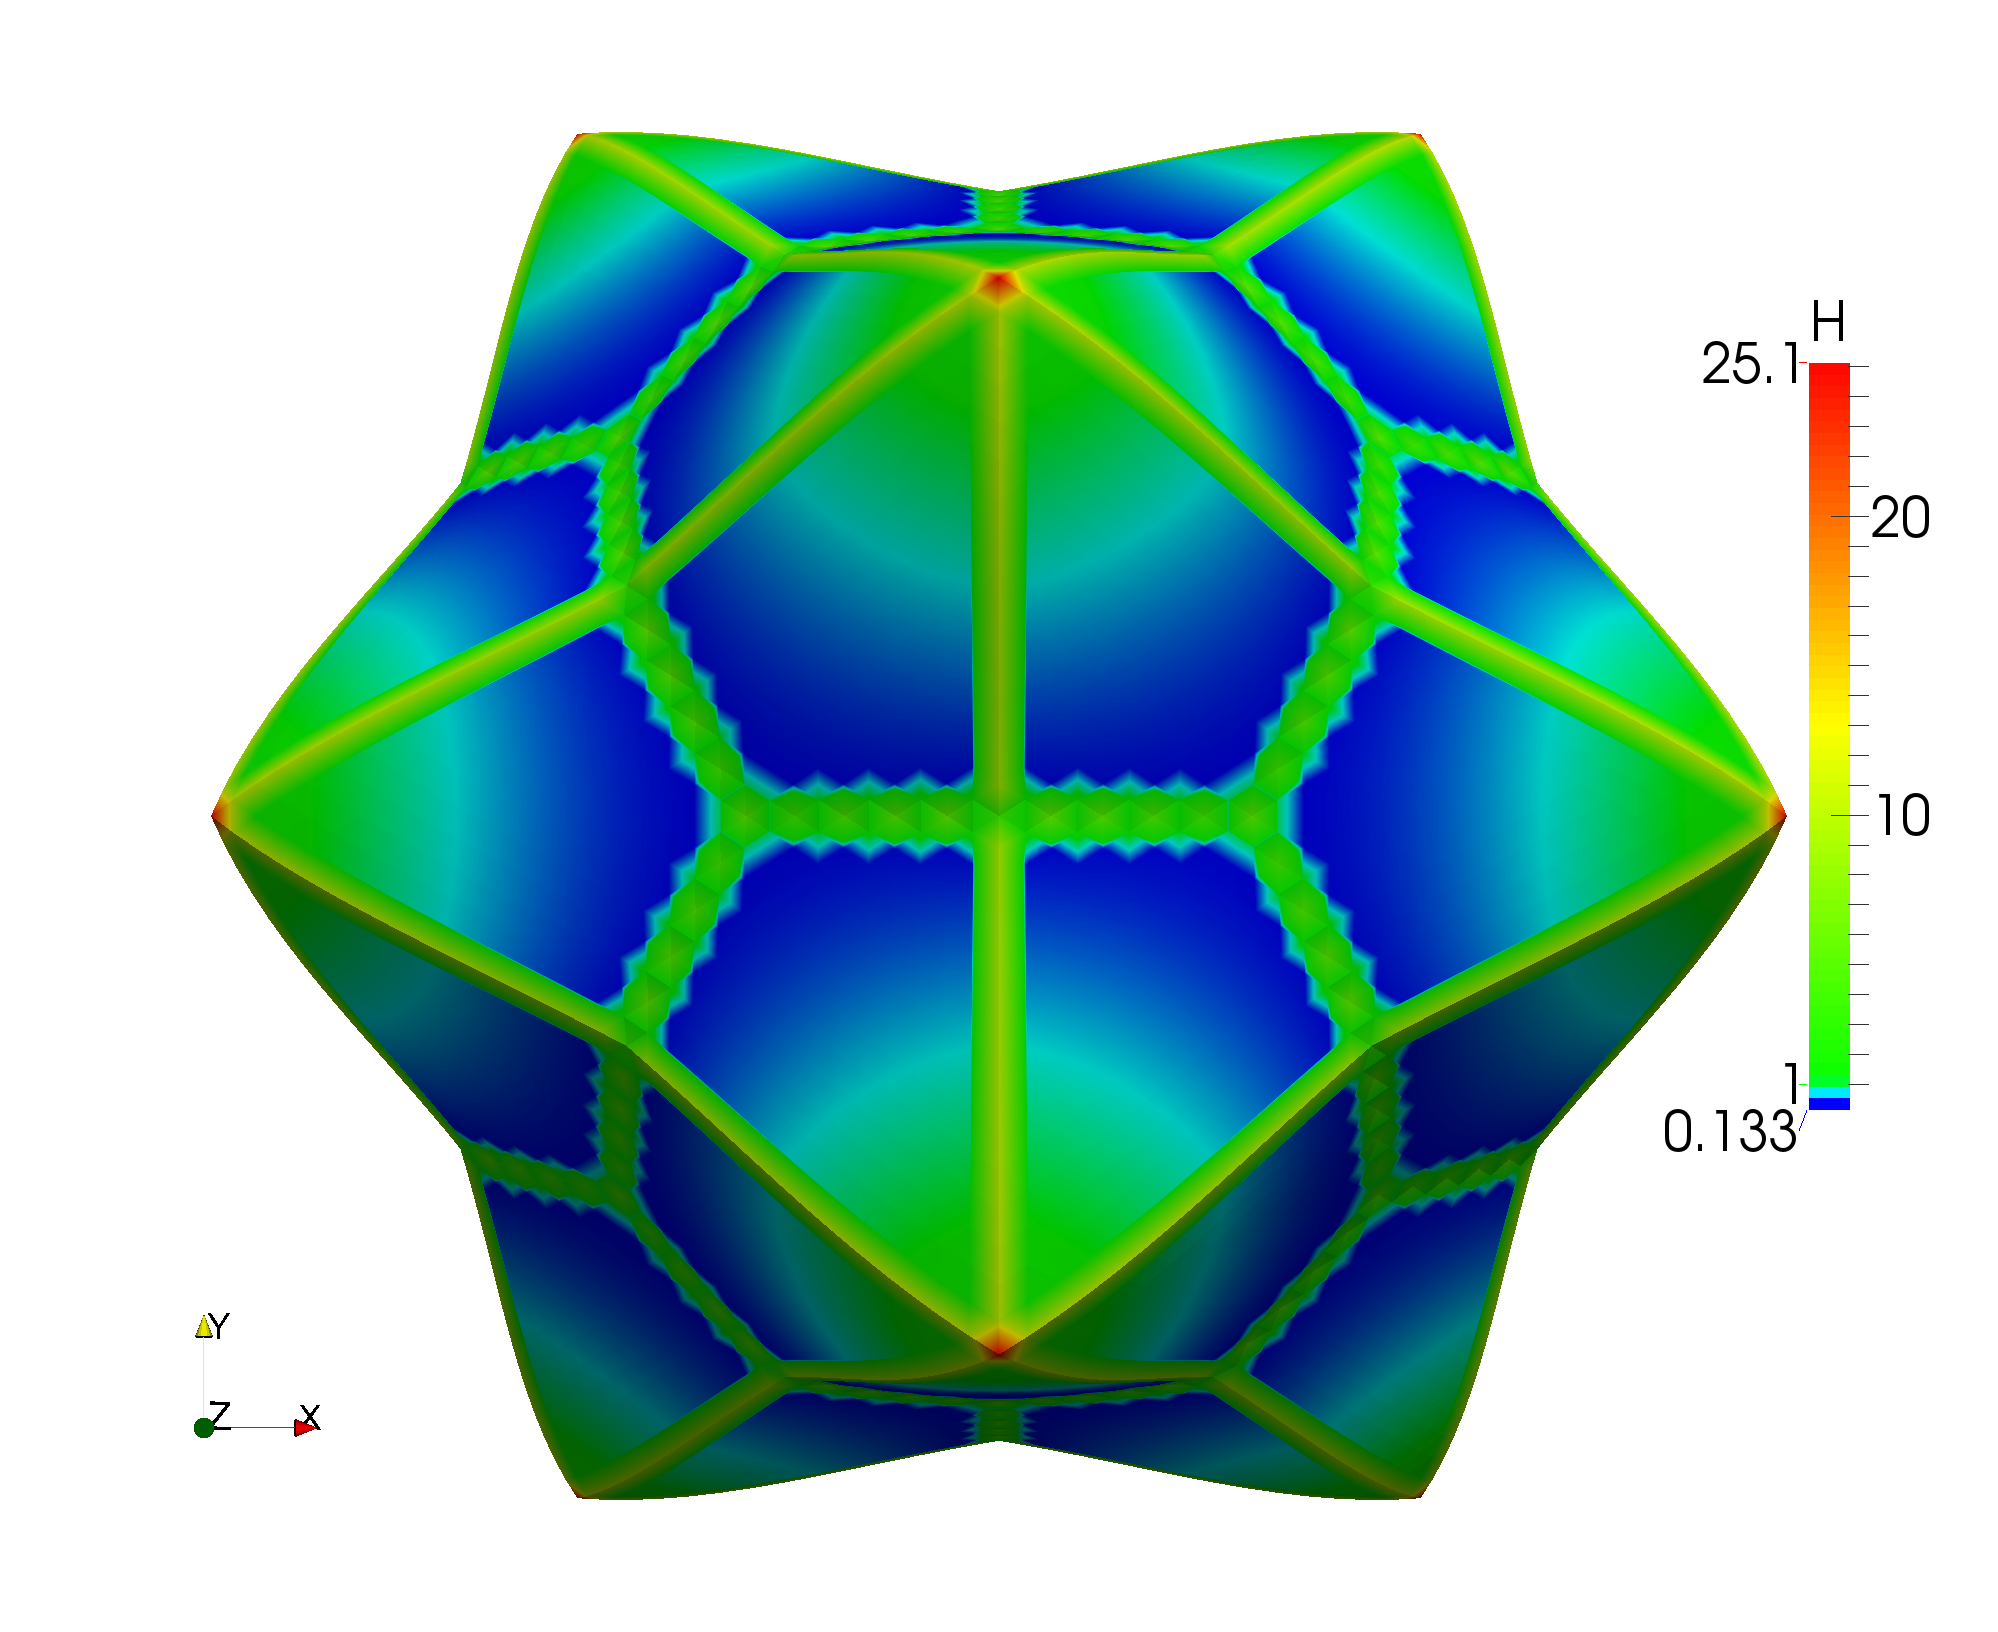
\includegraphics[width=\textwidth]{bilder/DefSphereMean.png}
    \end{minipage}\hfill
    \begin{minipage}[t]{0.24\textwidth}
       \centering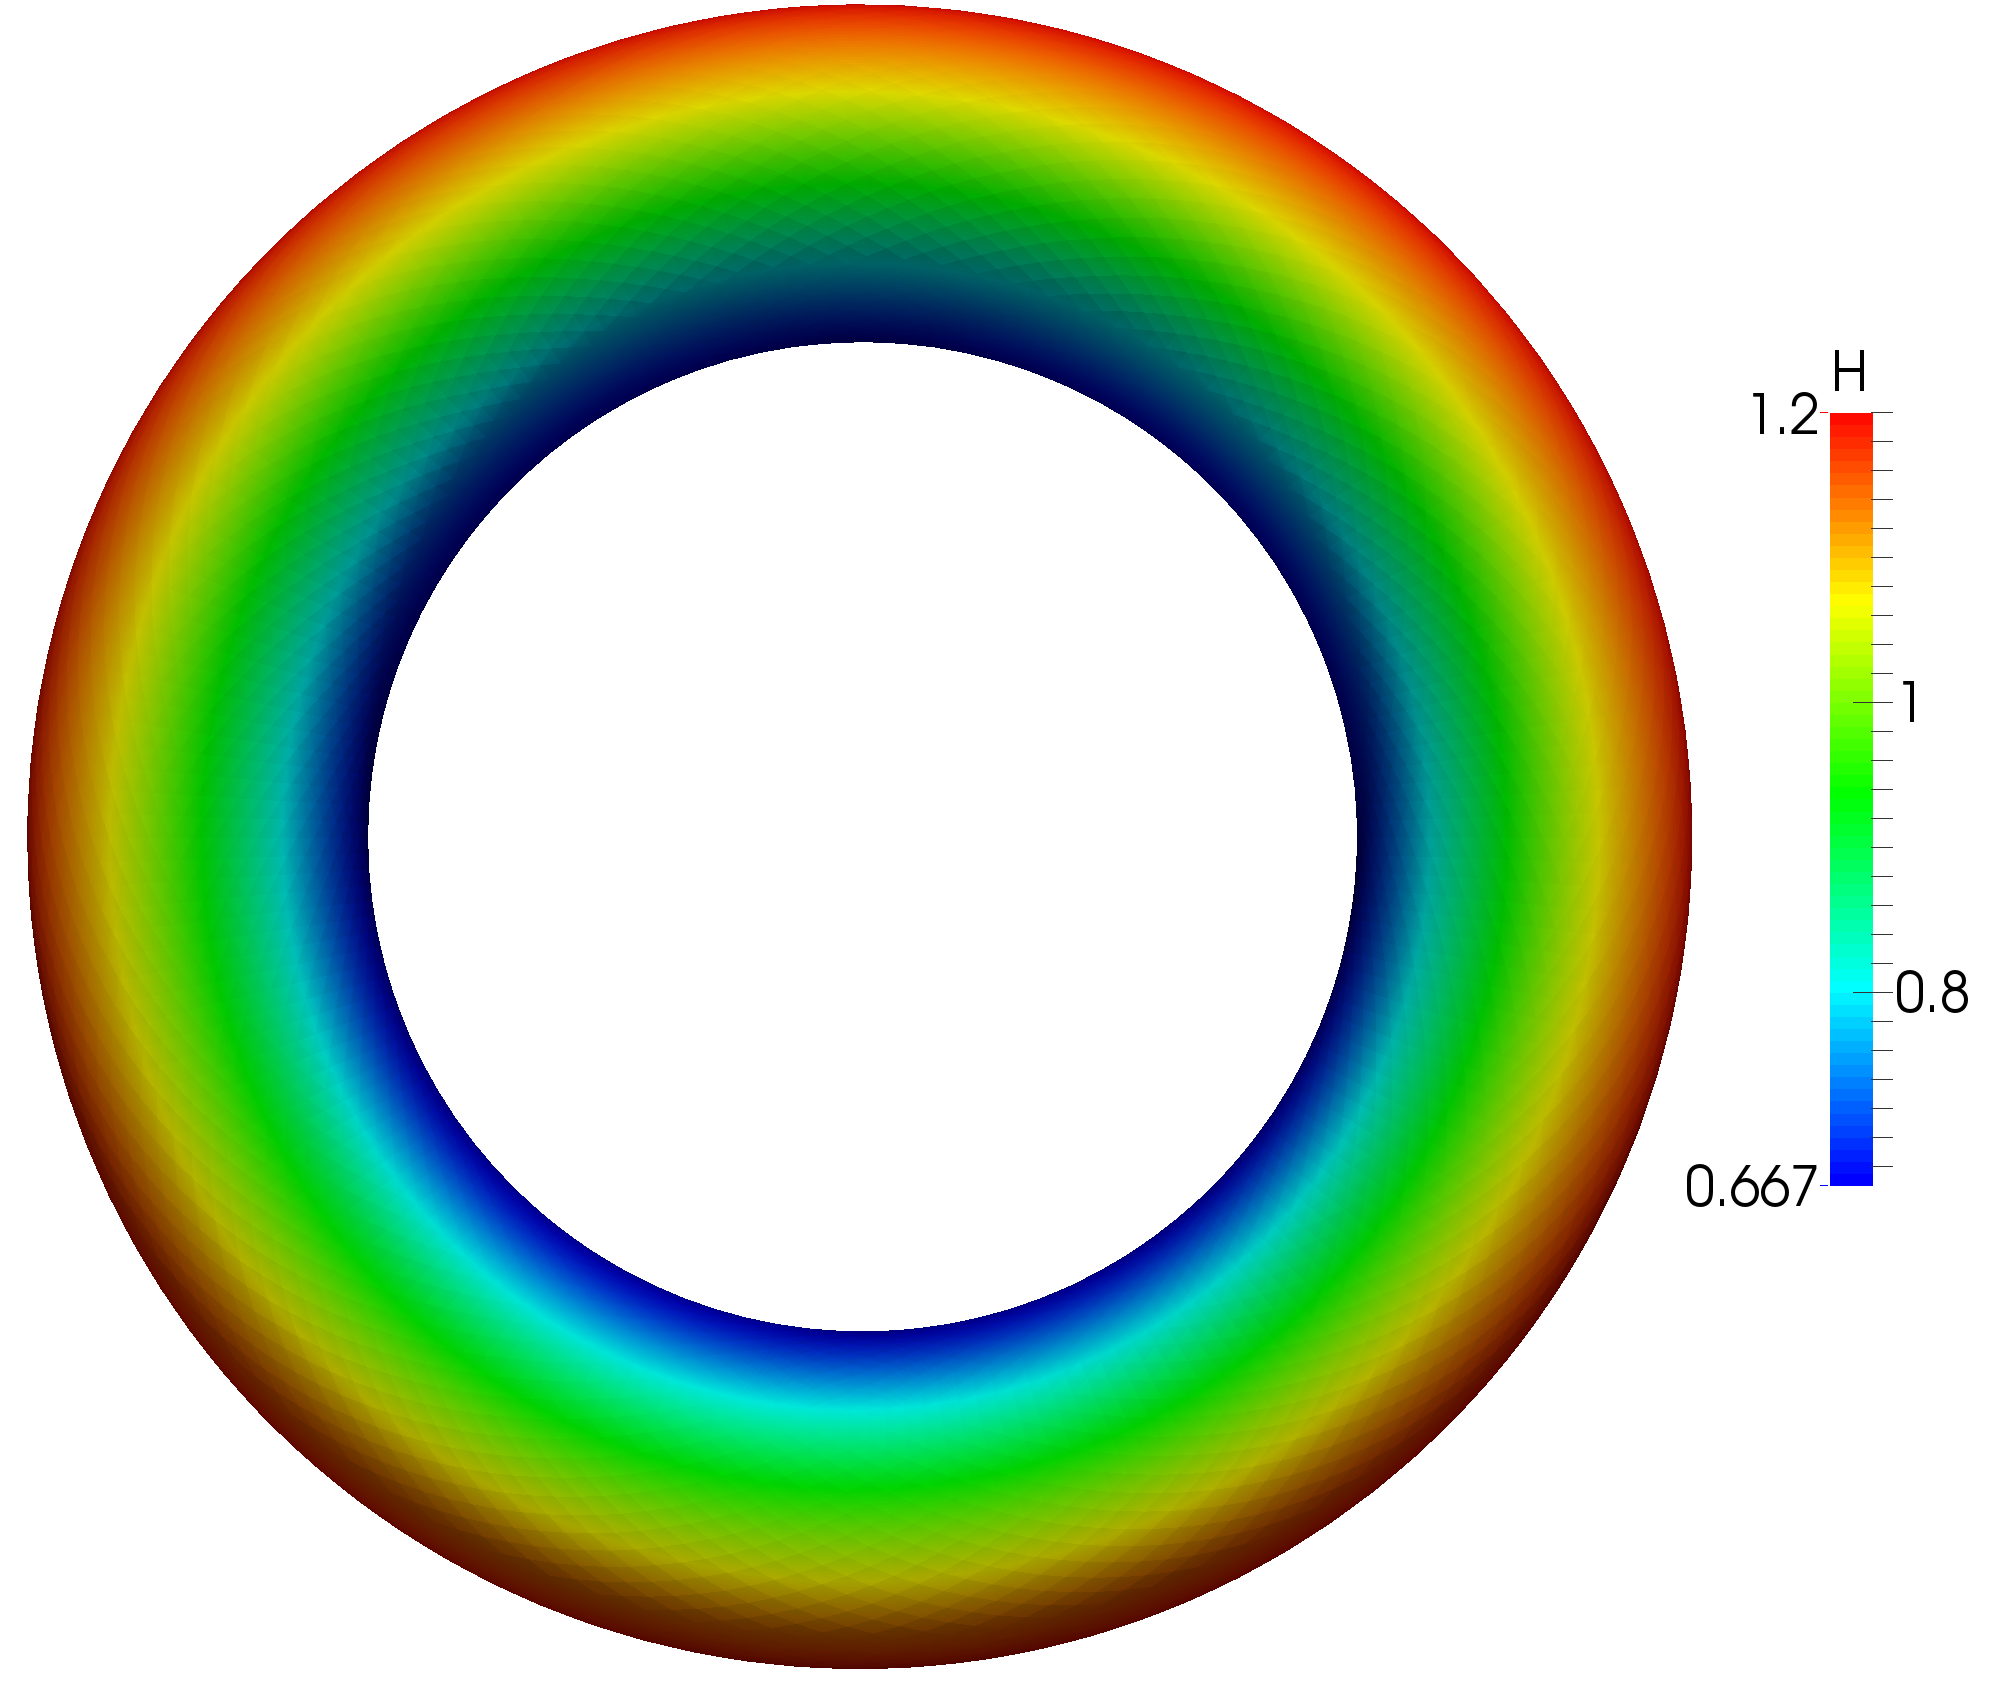
\includegraphics[width=\textwidth]{bilder/TorusMean.png}
    \end{minipage}
    \caption[Fehlerplot (Krümmungen auf Sphäre)]
            {Mean curvature of a ellipsoid, a quartic surface (\( \varphi(x,y,z) :=  (x-z^{2})^{2} + (y-z^{2})^{2} + z^{2} - 1 \)),
             a handmade surface (merge of a sphere and a icosahedron) and a torus.}
\end{figure}


\pagebreak
\nocite{flanders}\nocite{hirani}\nocite{heine}
\bibliographystyle{alpha}
\bibliography{../bibl.bib}{}
\end{document}
